\section{带余除法与同余} \label{sec:modulo}

在编程语言中有一个运算符``a\%b'',
可以计算一个数a被另一个数b除的余数,
称为取余运算或取模\footnote{模, modulus/modulo的音译.}运算.
虽然取余运算本身是确定的, 但各种应用场景对取余有不同的需求,
演化出各种变体的取余形式.
所以这一节讲一讲取余.

说到取余运算, 首先得从带余除法说起.
我们在小学应该学习过带余除法, 也就是
``$被除数 = 除数 \times 商 + 余数$''.
这个余数就是取余运算的输出结果.
小学我们在带余依法中只考虑正整数,
扩展到实数就得到了标准的\footnote{
  实际上带余除法一般在数论中讨论, 而数论中只考虑整数不考虑小数.
  后面的同余也是, 在数学上默认只考虑整数.
}带余除法定义:

\begin{definition}[带余除法]\label{def:divrem}
  对于任意两个数$a,b$ (其中$b>0$), 存在唯一一组数$q,r$使得
  \begin{equation}\label{eq:divrem}
    a = q \cdot b + r,
  \end{equation}
  其中$q$为整数, 且$0 \le r < b$.
  在上式中, $a$称为被除数, $b$称为除数, $q$称为商, $r$称为余数.
\end{definition}

具体怎么计算$q,r$呢?
考虑把\ref{eq:divrem}式做一个变形:
\[
  \dfrac ab = q + \dfrac rb.
\]
其中$a/b$是一个实数, $q$是一个整数, $r/b$是一个满足
$0 \le r/b < 1$的实数. 这是一个取整的模型,
$q$可以由$a/b$以某种方式取整计算出来.
根据$r/b$的取值范围, 这是一个\emph{向下取整},
换言之, $q$是小于或等于$a/b$的最大整数,
数学上表示为$q=\lfloor{a/b}\rfloor$.
\footnote{
  $\lfloor...\rfloor$表示向下取整,
  类似地$\lceil...\rceil$表示向上取整.
}
计算出$q$后, 用$r=a-qb$就可以得到$r$.

\begin{example}
  $a=-7$对$b=4$的带余除法.

  计算$a/b=-1.75$, 向下取整得到商$q=\lfloor{-1.75}\rfloor=-2$.
  计算余数$r = a-qb = 1$.
\end{example}

\subsection{同余}

\emph{同余}描述了两个数之间的某种特殊的联系,
它的字面意思是``余数相同''.
同余有几种看起来不同的定义方式,
读者可以证明这些定义方式有相同的效果:

\begin{definition}[同余]
  给定正数$m>0$, 对于两个数$a,b$, 以下几个条件是等价的:
  \begin{enumerate}[label=\arabic*.]
    \item $a$被$m$除得的余数与$b$被$m$除得的余数相等;
    \item $a-b$是$m$的整数倍;
    \item 存在整数$k$, 使得$a = k \cdot m + b$.
  \end{enumerate}
  当$a,b$满足上述条件 (中的一个) 时,
  我们说\emph{$a,b$模$m$同余}, 记作
  \[ a \equiv b \pmod{m}. \]
  所有与$a$模$m$同余的数所组成的集合称为
  \emph{$a$的同余类} (模$m$的),
  记作$[a]$.
\end{definition}

\begin{remark}
  同余描述的是$a,b$两个数之间的关系$a \equiv b$,
  模数$m$只是这个特定关系的一个``参数''.
\end{remark}

\begin{example}[时间]
  时钟大概是日常生活中与同余最接近的东西了.
  下午1点 (13:00) 和半夜1点 (1:00) 在时钟上指的是同一个位置,
  不同日期的下午1点在时钟上也是同一个位置.
  对于时钟来说, 时间是一个循环,
  每过12个小时, 时针就会回到原来的位置.

  \begin{figure}[htbp]
    \centering
    
\includegraphics[width=4cm]{assets/coord/clock.png}
    \caption{时钟}
    \label{fig:clock}
  \end{figure}

  同余就是这个道理. 模数$m$相当于时钟的循环周期 (12小时),
  $a,b$同余, 相当于时针指向同一个位置.
  在上面的例子中, 我们就可以说13与1是模12同余的.

  如果有人问你: ``现在是几点?''
  你回答``现在是1点''(假设你们使用12小时制).
  在做出这个回答时, 你并不关心究竟是哪一天的1点,
  也不管到底是下午的1点还是半夜的1点.
  同余类就是这个道理. 它不关心一个数值具体是多少,
  只关心模$m$下的哪个数能够代表它.
  在上面的例子中, 我们可以说1点就是模12的同余类$[1]$.
\end{example}

\begin{example}[任意角]
  给定一个角的始边和终边, 这个角的所有可能取值相差360\degree 的整数倍,
  这其实就是说所有的可能取值是模360\degree 同余的,
  或者说, 组成一个模360\degree 的同余类.
  为了表示一个完整的360\degree 范围,
  我们有时说$-180\degree \le \theta < 180\degree$,
  有时说$0\degree \le \theta < 360\degree$.
  从同余类的角度, 这些说法没有实际区别,
  只不过是用不同的具体数值来代表它们所在的同余类而已.
\end{example}

接下来简单说一说同余的性质.
如果是在一个正常的数学教程,
那么我应该在这之前做大量的数论内容的铺垫,
然后才能推进到同余的性质.
但是这里不是一个正常的数学教程,
或者说, 我们所在的不是一个纯粹的数学环境,
而是以编程/弹幕制作为主体的环境.
本来这一节的带余除法和同余都是数论中的概念,
在数论中只考虑整数而不考虑小数,
但在弹幕制作中很少会出现只讨论整数的情况.
因此我们给出的这些概念都是扩展到实数范围的.
这会破坏掉很多因整数而成立的性质, 结果就是,
我们所讨论的同余只剩下了一些由整除直接推导的, 非常基础的性质
(以下表述中, 默认$m$为任意正数, 且$a \equiv b \pmod{m}$):
\begin{enumerate}[label=\arabic*.]
  \item $a \equiv a+m \pmod{m}$.
  \item 对任意$c>0$, 有
        $c \cdot a \equiv c \cdot b \pmod{c \cdot m}$.
  \item 若$m'>0$能整除$m$, 则有
        $a \equiv b \pmod{m'}$.
  \item 若$a_1 \equiv b_1, a_2 \equiv b_2 \pmod{m}$,
        则有\[a_1+a_2 \equiv b_1+b_2 \pmod{m}.\]
  \item 对任意整数$k$, 有
        $k \cdot a \equiv k \cdot b \pmod{m}$.
\end{enumerate}

以上性质的证明留作习题 (

既然数值能够进行加减乘除运算,
我们希望同余类也能进行加减乘除运算.
以加法为例, 对于两个模$m$同余类$[a],[b]$,
从$[a],[b]$各取一个数作加法,
所有可能的加法结果组成一个新的集合,
我们希望这个集合仍然构成一个模$m$同余类
(自然, 这个同余类就是$[a+b]$).

那么实际情况如何呢? 很遗憾,
在考虑小数的情况下, 只有加减法 (由性质4证明)
和与整数相乘 (由性质5证明) 能够正确地进行.
以角度的同余类 (模360\degree) 为例:
\begin{itemize}
  \item 加减法: 对于同余类$[\alpha],[\beta]$,
        加法和减法的结果仍然构成同余类:
        $[\alpha]\pm[\beta] = [\alpha\pm\beta]$.
  \item 与整数相乘: 对于同余类$[\alpha]$和整数$k$,
        两者相乘的结果仍然构成同余类:
        $k\cdot[\alpha] = [k\cdot\alpha]$.
        某种程度上, 这也是一种加减法.
  \item 与小数相乘: 由于把两个角相乘没什么实际含义,
        我们就只看实数和角度相乘的结果了.
        考虑$0.5$和$[0\degree]$相乘,
        $[0\degree]=\{0\degree,360\degree,-360\degree,
          720\degree,...\}$,
        那么相乘的结果为$\{0\degree,180\degree,-180\degree,
          360\degree,...\}$,
        然而$0\degree,180\degree$属于两个不同的同余类,
        这就破坏了结果应当是一个同余类的条件.
        除法实质上就是乘以倒数, 也就没什么讨论的必要了.
\end{itemize}

\subsection{带余除法的变体}

如果在同余类的角度上看, 带余除法有什么样的变体完全无所谓:
以除数$b$为模数, 被除数$a$和余数$r$必然是同余的.
但是毕竟在实际应用中, 我们还是需要落实到具体的数值.
带余除法变体的核心思想在于,
商$q$的取整方式与余数$r$的取值范围会互相影响.

\subsubsection{商的取整方式}

在带余除法$a=qb+r$中,
$q$是由$a/b$取整得到的.
标准定义 (定义\ref{def:divrem}) 下, $q$由$a/b$向下取整得到, 此时
\[
  \dfrac rb = \dfrac ab - q \implies
  0 \le \dfrac rb < 1 \implies
  0 \le r < b.
\]
这也是Lua语言采用的计算方式.

以 C, C++, Java, C\# 为代表的一系列编程语言
则使用另一种取整方式: 截断取整,
就是不论正负, 直接把小数数位丢弃 (计算机领域称之为截断),
只保留整数位. 比如, $-1.75$截断取整后就是$-1$.
在计算机中, 直接丢弃小数位比其他的取整方式更加容易.
此时, 当$a>0$时, $r/b=a/b-q$满足$0 \le r/b < 1$,
即$0 \le r < b$, 与标准定义相同;
但在$a<0$时, 余数的取值范围为$-b < r \le 0$.
余数的取值范围与$a$的正负性相关,
这种不统一的行为在部分应用场景中会带来问题.
比如, 在读取数组时, 有时希望把索引对数组长度取余使得索引不会越界,
这时如果索引为负数, 那么取余结果仍然是负数, 导致索引越界报错.

如果我们采用四舍五入取整会发生什么?
这时$r/b = a/b - q$满足$-0.5 \le r/b < 0.5$,
即$-b/2 \le r < b/2$. 这样的余数范围也有一些应用,
比如想要比较两个角度所指的方向有多接近,
直接作差不能完全体现接近程度
(比如$0\degree$和$361\degree$的方向其实只差$1\degree$),
这时就可以用这种取余方式把角度差对$360\degree$取余,
越接近$0\degree$, 两个角度方向就越接近.

\subsubsection{余数的取值范围}

有些时候, 标准定义的余数范围$0 \le r < b$不能满足我们的需求.
比如, 我们想比较两个方向的接近程度, 把两个方向角相减,
角度差可能是任意实数, 于是考虑将角度差对360\degree 取余
得到一个$0\degree \sim 360\degree$的角度.
如果角度差接近0\degree, 或者接近360\degree
(因为这俩是等价角), 那么我们判断两个方向是相近的.
这样虽然能实现目标, 但总会感觉不太直观,
如果能够让取余结果为$-180\degree \sim 180\degree$,
那么判断条件就会直观很多 (只判断是否接近0\degree).

我们考虑将标准定义\ref{def:divrem}中余数的取值范围
从$0 \le r < b$改为$c \le r < b+c$.
显然仍然有唯一一组$q,r$满足定义.
以下是一种计算$q,r$的具体思路:

由$a = q \cdot b + r$, 设$r' = r - c$, 则有
\[
  a - c = q \cdot b + r',\quad
  0 \le r' < b.
\]
于是用标准带余除法可以计算
$q = \lfloor{(a-c)/b}\rfloor, r = a - qb$
(或者$r' = (a-c) \luamod b, r = r' + c$).

\subsection*{习题}

\begin{enumerate}
  \item \comment{*}
        在LuaSTG中实现一个函数\raw{SubAngle(a1,a2)},
        计算\raw{a1}与\raw{a2}的角度差在
        $-180\degree \sim 180\degree$范围的等价角.
        在边界上返回$-180\degree$还是$180\degree$都可以.
        以下例子展示了调用该函数应当返回的结果:
        \begin{align*}
          \raw{SubAngle(12,0)}     & \to 12   \\
          \raw{SubAngle(0,12)}     & \to -12  \\
          \raw{SubAngle(-400,490)} & \to -170 \\
        \end{align*}
  \item \comment{这题和这一节的内容真的有关系吗*}
        图\ref{fig:1way-windmill}展示了一个转速为
        $144\degree/2帧$的1way风车弹代码,
        而它实际上呈现为一个转速为0的5way风车弹
        (我不想解释, 我也不想让你解释, 我想你应该明白怎么回事).

        \begin{figure}[htbp]
          \centering
          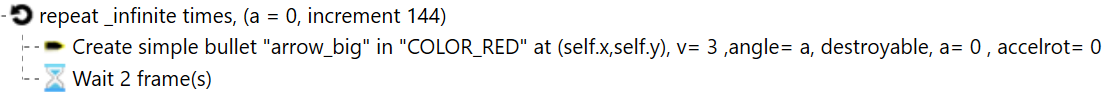
\includegraphics[width=\textwidth]
          {assets/coord/windmill.png}
          \caption{一个普通的1way(?)风车弹代码}
          \label{fig:1way-windmill}
        \end{figure}

        假设想让实际呈现的5way风车弹以$1\degree/2帧$的转速进行旋转,
        那么实际代码中\raw{a}在每轮循环的增量应该由144改为多少?
  \item \comment{这已经不是题了吧喂}
        锑块大佬对波粒的解析很不错的, 安利一波.

        \hyperlink
        {https://www.bilibili.com/video/BV1B7411m7tz/}
        {\textcolor{blue}
          {波与粒的境界为什么长这样？这个视频会告诉你一切}}

        \hyperlink
        {https://www.bilibili.com/video/BV1aQ4y1M7xh/}
        {\textcolor{blue}
        {对东方符卡的函数图像分析——[波与粒的境界]为什么长这样02}}
\end{enumerate}
